%===============================================================================
\section{Revisión de Estadística}
%===============================================================================

%-----------------------------------------------------------------
\subsection{Estimadores y propiedades}
%-----------------------------------------------------------------
\begin{frame}{Estimadores}
	\begin{itemize}
		\item Un estimador es la aproximación a parámetros o momentos poblacionales.
		\item Un estimador es una función de datos.
		\item Denotamos un estimador como un "sombrero".
		\item ¿Cómo elegimos un estimador? Debemos ocuparnos de lo siguiente
			\begin{itemize}
				\item Nos gustaría tener la siguiente propiedad: imparcialidad (es decir, $E (\hat{y}) = \mu_{Y})$
				\item Otra propiedad deseable: eficiencia (la más pequeña
				diferencia).
			\end{itemize}
	\end{itemize}
\end{frame}
%------------------------------------------------
\begin{frame}{Propiedades}
	Nos gustaría tener las siguientes propiedades para un buen estimador
		\begin{itemize}
			\item El sesgo de $\hat{y}$ es $E (\hat{y}) - \mu_{Y}$
			\item Sea $\tilde{y}$ o $\tilde{\mu}_{Y}$ otro estimador de $\mu_{Y}$ y supongamos que ambos estimadores son insesgados. Entonces, se dice que $\hat{y}$ es más eficiente que $\tilde{y}$ si var$(\hat{y}) <$ var$(\tilde{y})$
		\end{itemize}
	Tenga en cuenta que un estimador insesgado es consistente pero lo contrario no se cumple.
\end{frame}
%------------------------------------------------
\begin{frame}{Propiedades MELI}
	Algunos ejemplos. Vamos a considere los siguientes estimadores $\hat{\mu}_{Y^{j}}$ de $\mu_{Y}$. Compare los siguientes estimadores en términos de insesgadez y eficiencia.
		\begin{itemize}
			\item $\hat{\mu}_{Y^{0}}= \overline{Y} \equiv \frac{\sum \limits_{i=1}^{n}y_{i}}{n} $
			\item $\hat{\mu}_{Y^{1}}= \sum \limits_{i=1}^{n}y_{i}$
			\item $\hat{\mu}_{Y^{2}}= \sum \limits_{i=0}^{n}\omega^{i}y_{i}$ donde $\omega$ es una ponderación entre 0 y 1.
			\item $\hat{\mu}_{Y^{3}}= \sum \limits_{i=1}^{n}\lambda_{i}y_{i}$ donde $\sum_{i=0}^{n}\lambda_{i}=1$
		\end{itemize}
	Todas las variables aleatorias son i.i.d.(\textit{idéntica e independientemente distribuida})
\end{frame}

%-----------------------------------------------------------------
\subsection{Momentos muestrales}
%-----------------------------------------------------------------
\begin{frame}{Varianza muestral}
	la varianza es calculada como sigue
		$$ s_{Y}^{2} = \frac{\sum \limits_{i=1}^{n}(y_{i}-\overline{Y})^2}{n-1}$$ 
	la varianza de la muestra será útil para probar hipótesis. La desviación estándar de la muestra $(s_{Y})$ es la raíz de la varianza de la muestra
\end{frame}

%-----------------------------------------------------------------
\subsection{Prueba de Hipótesis}
%-----------------------------------------------------------------
\begin{frame}{Ho versus Ha}
	La hipótesis nula $(H_0)$ se especifica para la prueba. La hipótesis alternativa $(H_1 o H_a)$ se cumple si la nula no lo hace. En general, la hipotesis bilateral se configura como
		\begin{align*}
			&H_0 : E(x) = b\\
			&H_1 : E(x) \neq b
		\end{align*}
	La hipótesis unilateral se establece como
		\begin{align*}
			&H_0 : E(x) = b\\
			&H_1 : E(x) < b
		\end{align*}
	donde b es una escalar. En general, para probar la hipótesis nula, reemplazamos la media de la población con una estimación (por ejemplo, $\overline{x}$). Debemos concluir entre rechazar o no rechazar la hipótesis nula.
\end{frame}
%------------------------------------------------
\begin{frame}{Nivel de significancia}
	\begin{itemize}
		\item Es el tamaño de la prueba. Se denota como $\alpha$. Es el área de rechazo propuesta por el investigador.
		\item Eso nos da un umbral para rechazar o no rechazar la hipótesis nula.
		\item No confunda este término con la probabilidad de significancia o el p-value.
		\item Los valores estándar son: 0,01; 0.05 y 0.10
			\begin{itemize}
				\item si eliges valores más altos, más probabilidad de rechazar el nulo. Pero si el nulo es verdadero, tenemos problemas (Error tipo I, denotamos este error como $\alpha$)
				\item si eliges valores más pequeños, mayor probabilidad de no rechazar el nulo. Pero si el nulo es falso, tenemos problemas (Tipo de error II, denotamos este error como $1-\alpha$)
			\end{itemize}
	\end{itemize}
\end{frame}
%------------------------------------------------
\begin{frame}{El p-value}
	\begin{itemize}
		\item Stock y Watson (2011) afirman: ``Es la probabilidad de obtener una estadística al menos tan adversa a la hipótesis nula como la que realmente calculó en su muestra, asumiendo que la hipótesis nula es correcta''.
		\item Como profesor, digo ``Es la probabilidad más pequeña de rechazar la hipótesis nula''.
		\item Como alummno, digo  ``Es la probabilidad de obtener valores superiores a la estimación''.
		\item Debe contrastar el valor p con el nivel de significancia (?). Por lo tanto, tenemos que si 
			$$p-value < \alpha$$
		Entonces debes rechazar la hipótesis nula; de manera equivalente, puede decir ``Hay evidencia en la muestra para rechazar el Ho''
	\end{itemize}
\end{frame}
%------------------------------------------------
\begin{frame}{El p-value}
	Debes considerar la distribución y el tipo de $H_o$ que vas a probar:\\
		\medskip
		{\small{\centering
		\begin{tabular}{ccc} 
			\hline
				Distribución & Lados & P-valor\\
			\hline
					\addlinespace[1ex]
				N		 & Uno & Pr$\left(\frac{X-b}{\sigma_{\hat{x}}} < \frac{\hat{x}-b}{\sigma_{\hat{x}}} \right)$ or Pr$\left(\frac{X-b}{\sigma_{\hat{x}}} > \frac{\hat{x}-b}{\sigma_{\hat{x}}} \right)$\\
					\addlinespace[1ex]
				{}       & Dos & 2$\cdot \left[ \textup{Pr}\left(\frac{X-b}{\sigma_{\hat{x}}} > \left|  \frac{\hat{x}-b}{\sigma_{\hat{x}}}\right| \right)\right] $\\
					\addlinespace[1ex]
			\hline
					\addlinespace[1ex]
				$\chi^2$ & Uno & $\textup{Pr}\left(\chi^{2} > \hat{\chi}^{2} \right) $\\
					\addlinespace[1ex]
			\hline
					\addlinespace[1ex]
				F		 & Uno & $\textup{Pr}\left( F > \hat{F} \right) $\\
					\addlinespace[1ex]
			\hline
					\addlinespace[1ex]
				t		 & Uno & Pr$\left(\frac{X-b}{\sigma_{\hat{x}}} < \frac{\hat{x}-b}{\sigma_{\hat{x}}} \right)$ or Pr$\left(\frac{X-b}{\sigma_{\hat{x}}} > \frac{\hat{x}-b}{\sigma_{\hat{x}}} \right)$\\
					\addlinespace[1ex]
				{}       & Dos & 2$\cdot \left[ \textup{Pr}\left(\frac{X-b}{\sigma_{\hat{x}}} > \left|  \frac{\hat{x}-b}{\sigma_{\hat{x}}}\right| \right)\right] $\\
					\addlinespace[1ex]
			\hline
		\end{tabular}}\\}
	\medskip
	Donde $X$ se distribuye como $N(b,\sigma_{x}^{2})$
\end{frame}
%------------------------------------------------
\begin{frame}{El p-value}
	\begin{figure}
		\centering
		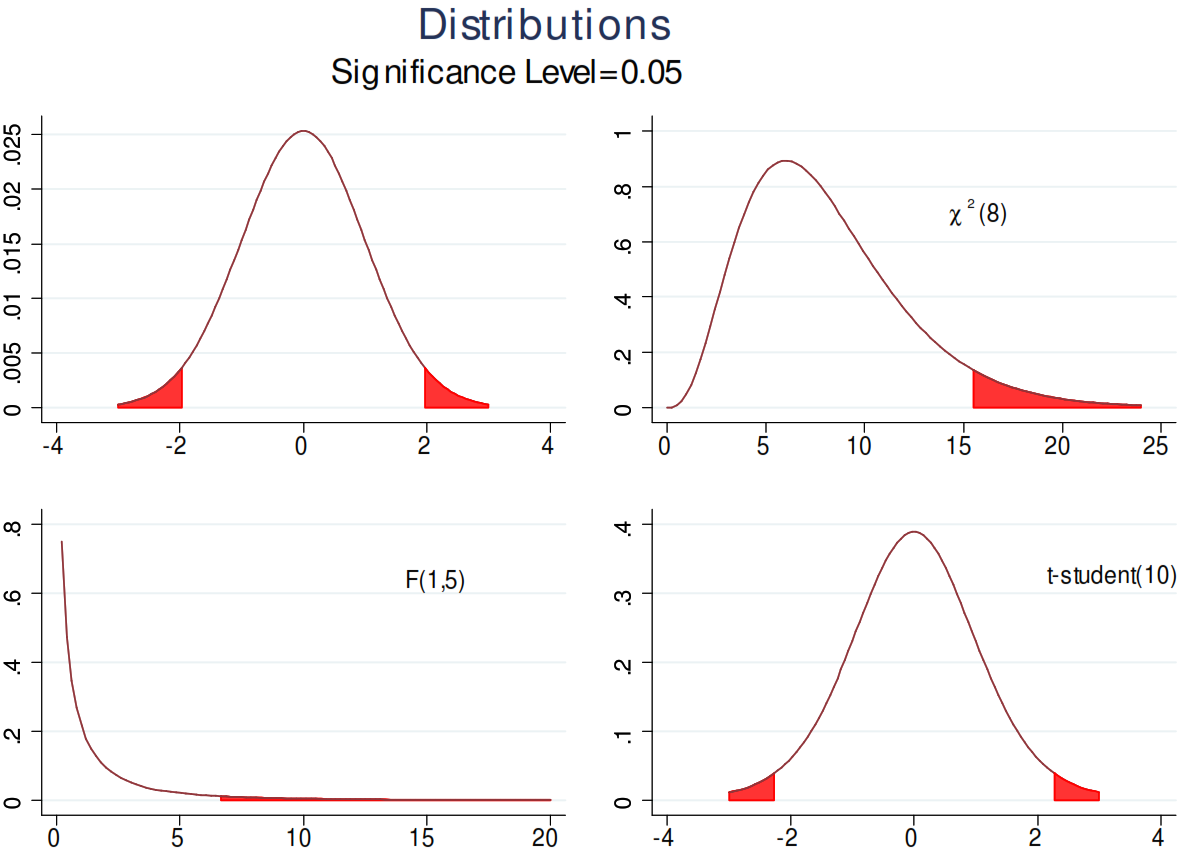
\includegraphics[scale=.30]{figuras/pvalue.png}
	\end{figure}
\end{frame}
%------------------------------------------------
\begin{frame}{Ejemplo}
	\begin{itemize}
		\item Un estudiante de una clase de econometría realiza una prueba estadística en sus calificaciones. Este alumno configuró el siguiente $Ho: \overline{Y} = 70$. La distribución de sus calificaciones -basada en el desempeño pasado- se considera normal con media 50 y varianza 6.
		\item Sean $y_1, y_2 \ldots y_n$ i.i.d se extrae de una distribución con media $\mu_{Y}$. Una prueba de $H_0: \mu_{Y} = 5; H1: \mu_{Y} \neq 5$ utilizando el estadístico t habitual produce un valor p de 0,03. ¿Cuál es la conclusión de la prueba?.
	\end{itemize}
\end{frame}
%------------------------------------------------
\begin{frame}{El p-value}
	\begin{itemize}
		\item ¿Qué es el P-Value?
		\item Definición formal:
				{\centering \textit{``es la probabilidad de obtener un efecto por lo menos tan extremo como el de los datos de la muestra, asumiendo que la hipótesis nula es verdadera.''}}
		\item ¿Se entiende?
		\item Déjenme intentar con una aproximación distinta usando un caso de la vida real.
	\end{itemize}
\end{frame}
%------------------------------------------------
\begin{frame}{El p-value}
	La escena del crimen
	\begin{figure}
		\centering
		
\includegraphics[scale=.30]{figuras/pvalue1.png}
	\end{figure}
\end{frame}
%------------------------------------------------
\begin{frame}{El p-value}
	Lo correcto en cualquier juicio es asumir inocencia (Paso 1: hipótesis nula).
	\begin{figure}
		\centering
		
\includegraphics[scale=.30]{figuras/pvalue2.png}
	\end{figure}
\end{frame}
%------------------------------------------------
\begin{frame}{El p-value}
	Esto obliga a definir un conjunto de posibilidades en las que el cachorro es inocente aunque algunas de ellas sean poco probables (Paso 2: Modelo matemático)
	\begin{figure}
		\centering
		
\includegraphics[scale=.30]{figuras/pvalue3.png}
	\end{figure}
\end{frame}
%------------------------------------------------
\begin{frame}{El p-value}
	Usar la evidencia para concluir algo (Paso 3: Contrastación)
	\begin{figure}
		\centering
		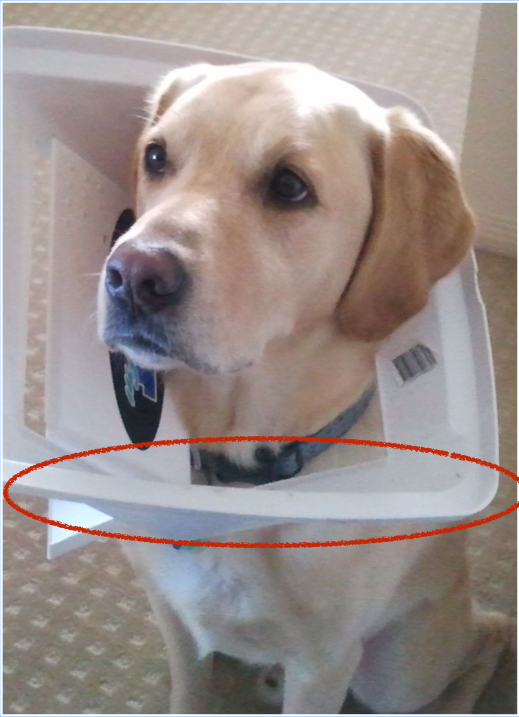
\includegraphics[scale=.30]{figuras/pvalue4.png}
	\end{figure}
\end{frame}
%------------------------------------------------
\begin{frame}{El p-value}
	Analogía con un juicio
		\begin{itemize}
			\item ¿Cuál es la hipótesis en un juicio?
					$$Inocencia\enskip (hipótesis\enskip nula) $$
			\item ¿Cuál es el rol de un ?scal?
					$$Rechazar\enskip la\enskip nula.$$
			\item Pero el ?scal siempre tiene un margen de error. 
			\item La probabilidad de error al tratar de rechazar la nula es el P-Value.
		\end{itemize}
\end{frame}
%------------------------------------------------
\begin{frame}{El p-value}
	El fiscal siempre rechaza la nula, la diferencia está en el p-value
		\begin{itemize}
			\item Si Fiscal señala que el error es de 0.00001\%.
			\item Si Fiscal señala que comete un error de 99.99\%.
		\end{itemize}
\end{frame}
%------------------------------------------------
\begin{frame}{El p-value}
	\begin{itemize}
		\item Y si el fiscal dice que el error es de 20\%...
		\item ¿Cuál es el máximo error que están dispuestos a tolerar para estar de acuerdo con el fiscal? ¿1\%?; ¿5\%?; ¿10\%?
		\item Dicho umbral o tolerancia se le conoce como \textbf{NIVEL DE SIGNIFICANCIA}, es subjetivo y depende del analista y del problema que se esté analizando.
		\item ``No es igual un p-value de 10\% en un experimento médico que en un paper universitario''.
	\end{itemize}
\end{frame}
%------------------------------------------------
\begin{frame}{EL p-value}
	Para concluir algo respecto a una hipótesis sólo se requieren de dos elementos:
		\begin{enumerate}
			\item Conocer la hipótesis
			\item Identificar el p-value asociado a la hipótesis
		\end{enumerate}
	Que este valor sea pequeño o grande depende del analista, aunque es usual compararlo con los niveles de 1\%, 5\% y 10\%.
\end{frame}
%------------------------------------------------
\begin{frame}{Conclusiones}
	Debes tener en cuenta los siguientes pasos para tener una puntuación completa:
		\begin{enumerate}
			\item Escriba la hipótesis nula y alternante.
			\item Elija el nivel de significancia o $\alpha$.
			\item Elija la prueba correctamente (y la distribución relacionada)
			\item Determine el área de rechazo (de acuerdo con la configuración realizada en el paso 1)
			\item Calcule el estadístico.
			\item ¡Y da la conclusión !. (¡PASO muy importante!)
		\end{enumerate}
\end{frame}

%-----------------------------------------------------------------
\subsection{Intervalo de confianza}
\begin{frame}{Un intertvalo de confianza}
	\begin{itemize}
		\item Se construye un intervalo de confianza alrededor de la estimación y ese conjunto indica todos los valores posibles donde se encuentra el valor real de la media de la población o parámetro (o estimación insesgada); por supuesto con alguna probabilidad de ocurrencia.
		\item Las probabilidades estándar son 99, 95 y 90\%.
		\item Un intervalo de confianza no significa precisión, significa confianza donde se encuentra el verdadero parámetro.
		\item En la página 80, Stock y Watson afirman que \textit{``Un intervalo de confianza de dos lados del 95\% para $\mu_{Y}$ es un intervalo construido para que contenga el verdadero valor de $\mu_{Y}$ al 95\% de todas las muestras aleatorias posibles''}.
	\end{itemize}
\end{frame}
%------------------------------------------------
\begin{frame}{Una notación alternativa para intervalos de confianza}
	Aquí una alternativa y asumiendo normalidad
		\begin{align*}
			& 90\% \textup{ I.C. para} \mu_{Y} =[\hat{\mu}_{Y} \pm 1.64 \cdot \hat{\sigma}_{\mu_{Y}}] \equiv [\overline{\mu_{Y}}; \underline{\mu_{Y}}]_{90\%}\\
			& 95\% \textup{ I.C. para} \mu_{Y} =[\hat{\mu}_{Y} \pm 1.96 \cdot \hat{\sigma}_{\mu_{Y}}] \equiv [\overline{\mu_{Y}}; \underline{\mu_{Y}}]_{95\%}\\
			& 99\% \textup{ I.C. para} \mu_{Y} =[\hat{\mu}_{Y} \pm 2.58 \cdot \hat{\sigma}_{\mu_{Y}}] \equiv [\overline{\mu_{Y}}; \underline{\mu_{Y}}]_{99\%}
		\end{align*}
	Pregunta: ¿qué son esos valores 1,64, 1,96 y 2,58 ?. Respuesta: Estimado alumno, son valores críticos.
\end{frame}

%-----------------------------------------------------------------
\subsection{Comparando promedios de poblaciones similares y diferentes}
%-----------------------------------------------------------------
\begin{frame}{Comparando promedios de poblaciones diferentes}
	La $H_0$ y $H_1$ en este caso son:
		\begin{align*}
			& H_0 : \mu_{POP1} - \mu_{POP2} = d \\
			& H_1 : \mu_{POP1} - \mu_{POP2} \neq d
		\end{align*}
	El estadístico $t$ (asumiendo muestras pequeñas) es
		$$t=\frac{\hat{\mu}_{POP1} - \hat{\mu}_{POP2} - d}{\sqrt{\frac{\hat{S}_{POP1}^{2}}{n_{POP1}}+\frac{\hat{s}_{POP1}^{2}}{n_{POP2}}}}$$
\end{frame}
%------------------------------------------------
\begin{frame}{Comparando promedios de poblaciones similares}
	La $H_0$ y $H_1$ en este caso son:
		\begin{align*}
			& H_0 : \mu_{POP1} - \mu_{POP2} = d \\
			& H_1 : \mu_{POP1} - \mu_{POP2} \neq d
		\end{align*}
	En este caso las varianzas son las mismas(Misma población)
	$$t=\frac{\hat{\mu}_{POP1} - \hat{\mu}_{POP2} - d}{\hat{S}\sqrt{\frac{1}{n_{POP1}}+\frac{1}{n_{POP2}}}}$$
	Y el error estandar se calcula como:
	$$\hat{s}^{2}=\frac{1}{n_{POP1} + n_{POP1} -2}\left[ \sum \limits_{i=1}^{n_{POP1}} (y_{POP1, i}-\hat{\mu}_{POP1})^2+
	\sum \limits_{i=1}^{n_{POP2}}(y_{POP2, i}-\hat{\mu}_{POP2})^2 \right]$$
\end{frame}